
%(BEGIN_QUESTION)
% Copyright 2012, Tony R. Kuphaldt, released under the Creative Commons Attribution License (v 1.0)
% This means you may do almost anything with this work of mine, so long as you give me proper credit

Suppose we have a Koyo ``CLICK'' PLC connected to three process switches as shown in this illustration:

$$\includegraphics[width=15.5cm]{i02145x01.eps}$$

Determine the process conditions (i.e. temperature, level, and pressure values) given the ``offline'' display of the ladder logic program shown here, knowing that the lamp happens to be {\it energized} at the present time:

$$\includegraphics[width=15.5cm]{i02145x02.eps}$$


\underbar{file i02145}
%(END_QUESTION)





%(BEGIN_ANSWER)

If the lamp is energized, we know that the top two virtual contacts ({\tt X1} and {\tt X2}) are colored, and/or the bottom two virtual contacts ({\tt X3} and {\tt X2}) are colored.

\vskip 10pt

For the top two virtual contacts to be colored, {\tt X1} must be 0 and {\tt X2} must be 1.  This equates to a pressure less than 32 PSI and a level less than 10 inches.

\vskip 10pt

For the bottom two virtual contacts to be colored, {\tt X3} must be 1 and {\tt X2} must be 0.  This equates to a temperature greater than 99 $^{o}$F and a level greater than 10 inches.

%(END_ANSWER)





%(BEGIN_NOTES)


%INDEX% PLC, relating I/O status to virtual elements 

%(END_NOTES)


